%  Created by Branden Stone on 2015-01-15.
%  Copyright (c) 2015 Branden Stone. All rights reserved.
%--------------------------------------------------------
\documentclass{exam}


%---------------------------
% Packages
%---------------------------
\usepackage{amssymb, amsmath, latexsym, amsfonts, amsthm, mathrsfs} % Standard packages that are nice to have.
\usepackage{amsrefs} % Allows for easy referencing and citations.
\usepackage{verbatim} % Needed for \begin{comment} \end{comment}.
\usepackage[text={6in,9in},centering]{geometry} % Defines the dimensions of the text body.
\usepackage[colorlinks=true]{hyperref} % Allows for use of hyperlinks.
%\usepackage[doublespacing]{setspace} % Makes the document double spaced.
\usepackage[pdftex]{graphicx} % Allows for \includegraphics

\addpoints

\newcommand{\lst}[2]{#1_1,\dots,#1_{#2}}

%----------------------------
% Title and Author
%----------------------------

\title{Math 390 Midterm}
\author{Due Friday, May 20}
\date{}


%----------------------------
% Main Document Body
%----------------------------

\begin{document}


%-------------------------------------------------------------
% Front Matter: This is where you can add a table of contents,
% preface, list of figures, ETC. for this template we will 
% only create a title and author name with `\maketitle'
%-------------------------------------------------------------

\maketitle

\setlength{\parindent}{0em} % Sets indentation of new paragraph
\setlength{\parskip}{1em} % Sets space between paragraphs

%-------------------------------------------------------------
% Document Body: Essentially this is where you place the 
% content of your document. To use this template, just delete
% all of the text between here and the Bibliography Section.
% Then type whatever you desire.
%-------------------------------------------------------------

You must work completely on your own, consulting only the textbook, your course notes, and your homeworks as references. Show all of your work. If you have questions, you can come to my office hours or ask me via e-mail. Solutions should be written in \LaTeX\ or Markdown and converted to a PDF. There are \numquestions\ questions for a total of \numpoints\ points. Good luck!

\begin{questions}

\question A graph $G$ is {\bf 1-Hamiltonian} if for all vertices $v\in V(G)$, the graph $G-v$ (obtained by deleting $v$ and the edges incident to $v$) is Hamiltonian.

\begin{parts}
	\part[15] For each of the following graphs, determine whether the graph is 1-Hamiltonian. Justify your answers.
		\begin{center}
			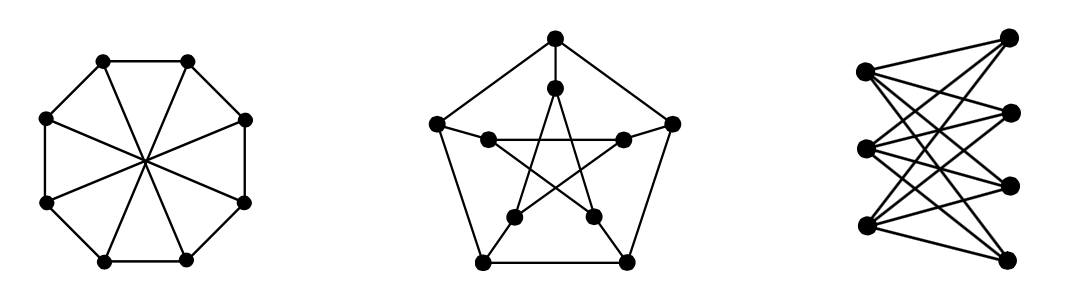
\includegraphics[width=0.6\textwidth]{finalpic1.png}
		\end{center}

	\part[6] Find a graph that is Hamiltonian but not 1-Hamiltonian.

	\part[9] Let $G$ be a 1-Hamiltonian graph and let $u$ and $v$ be two distinct vertices in $G$. Prove that there are at least three disjoint paths from $u$ to $v$.
\end{parts}

\question[15] The {\bf bipyramid} $B_n$ is the graph with $n$ vertices consisting of a cycle with $n-2$ vertices and 2 additional vertices that are both adjacent to all of the vertices in the cycle. The bipyramids $B_5$, $B_6$, and $B_7$ are shown below:
		\begin{center}
			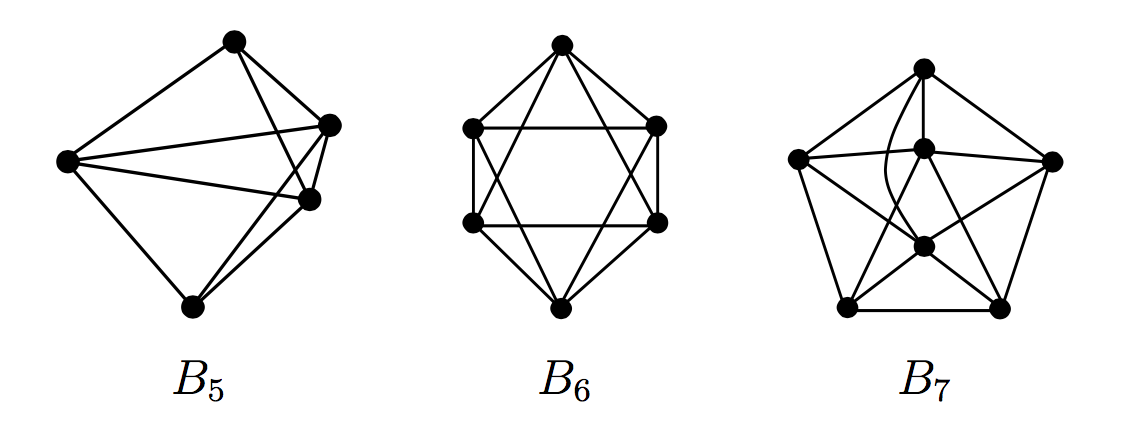
\includegraphics[width=0.6\textwidth]{finalpic2.png}
		\end{center}		
Determine the chromatic polynomial of $B_n$ for $n\geqslant 5$. Prove your answer.

\question[20] Let $G$ be a simple bipartite graph in which every vertex has degree $r$.
\begin{parts}
	\part Use Hall's Theorem to show that $G$ has a complete matching.
	\part Without using Theorem 20.4 from Edition 4 of the textbook or Theorem 5.18 from Edition 5 of the textbook, prove that the chromatic index of $G$ is $r$. (Hint: Use part (a).)
\end{parts}

\pagebreak

\question[15] Let $G$ be a simple bipartite graph with bipartition $A$ and $B$ in which every vertex in $A$ has degree at least $t$ with $t > |A|$, and suppose that $G$ satisfies the conditions of Hall's Theorem (every subset $X\subseteq A$ is adjacent to at least $|X|$ vertices in $B$). Since $t > |A|$, the graph $G$ will have multiple complete matchings from $A$ to $B$). Use induction on $|A|$ to show that $G$ has at least $\displaystyle \frac{t!}{(t - |A|)!}$ complete matchings from $A$ to $B$.


\question

\begin{parts}
	\part[5] We can write a minimal spanning tree of a graph by listing the edges of the tree. For example, $\{a, b, c\}$ is a minimal spanning tree of the graph below. Find all minimal spanning trees and write them as lists. Justify why you have all of them. (Hint: First count the number of minimal spanning trees, then find all of them. If only we had a theorem that would help us count them\ldots)

		\begin{center}
			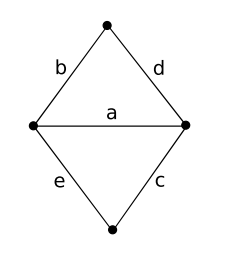
\includegraphics[width=0.2\textwidth]{finalpic4.png}
		\end{center}	

	\part[3] Let $\mathcal T$ be the set of all spanning trees of a the graph in part (a) (this is a list of lists). Define $\mathfrak T$ to be the set of all subsets of elements in $\mathcal T$. Determine $\mathfrak T$. 

	For example, if 
	\[
		\mathcal T = \{ \{1,2,3\}, \{3, 4\}\},
	\] 
	then 
	\[
		\mathfrak T = \{ \emptyset, \{1\}, \{2\}, \{3\}, \{4\}, \{1,2\}, \{1,3\}, \{2,3\}, \{3,4\}, \{1,2,3\} \}.
	\]
%	\[
%		\mathfrak T = \bigcup_{U \in \mathcal T} 2^U
%	\]
	
	\part[6] Let $G$ be a graph (not necessarily simple). Using the notation in part (b), show that for any two spanning trees, $S,T \in \mathcal T$, and an edge $e \in S$, we can always find some edge $f \in T$ such that $(S\setminus e)\cup f$  is also in $\mathcal T$. 

	\part[6] Let $G$ be a graph (not necessarily simple). Using the notation in part (b), show that for any two elements, $S,T \in \mathfrak T$ such that $|T| = |S|+1$, we can always find some element $f \in T\setminus S$ such that $S\cup f$ is also in $\mathfrak T$. {\it The edge set $E(G)$ together with the set $\mathfrak T$ is called a matroid and denoted $M = (E,\mathfrak T)$.}




\end{parts}



\end{questions}





\end{document}